\chapter{Experimentación}\label{cap:experimentacion}

\section{Experimentos preliminares}

En esta primera fase de experimentacion se realizarán pruebas para determinar los parámetros óptimos de ejecución y estudiar el rendimiento de la aplicación en distintos entornos y plataformas.

\subsection{Determinación del número óptimo de subpoblaciones y hebras}

Como se ha comentado en la sección \ref{subsubsec:determinacion_subpoblaciones}, se realizarán ejecuciones exploratorias con distintas configuraciones de subpoblaciones y hebras, para definir el parámetro de \texttt{NSubpopulations} a usar en los tests posteriores.

En la figura \ref{fig:exploratory_subpopulations} se muestran las gráficas de estas ejecuciones exploratorias. Se observa que para cualquier número de subpoblaciones, el comportamiento es similar. En la tabla \ref{tab:exploratory_subpopulations_times} se presentan los tiempos de ejecución en segundos para cada combinación de hebras y subpoblaciones, mostrando cómo el incremento en el número de subpoblaciones aumenta significativamente el tiempo de ejecución, especialmente cuando se utilizan pocas hebras.

En la tabla \ref{tab:exploratory_populations_delta} se presentan los porcentajes de reducción del tiempo de ejecución respecto a la configuración base. En cada columna, la ejecución con una sola hebra y una sola subpoblación se toma como referencia (0\% de reducción). Estos resultados permiten cuantificar de manera objetiva el beneficio relativo derivado del incremento del paralelismo y de la subdivisión de la población, proporcionando una base empírica para identificar configuraciones óptimas de ejecución.

Del análisis de esta tabla pueden extraerse varias conclusiones de interés para la definición de los parámetros en los experimentos posteriores. En primer lugar, se observa que, para un número fijo de hebras, la variación en el porcentaje de reducción del tiempo es prácticamente inexistente al modificar el número de subpoblaciones, lo que indica que el comportamiento es proporcional con independencia de este parámetro. En segundo lugar, el mayor beneficio en términos de reducción del tiempo de ejecución se obtiene al incrementar el número de hebras de 1 a 8, alcanzando valores en torno al 83--84\%. Sin embargo, al pasar de 8 a 16 hebras, los tiempos de ejecución se incrementan en todos los casos, lo que revela que se ha sobrepasado el punto de paralelismo óptimo para la arquitectura hardware utilizada. Este resultado sugiere que, en el entorno experimental considerado, el uso de más de 8 hebras no proporciona mejoras de rendimiento adicionales e, incluso, puede resultar contraproducente debido a la sobrecarga y la contención de recursos.

No obstante, se ha decidido mantener configuraciones con 16 hebras en los experimentos posteriores con el fin de analizar el comportamiento bajo condiciones de sobrecarga, dado que el objetivo del estudio trasciende la mera optimización de un caso específico y busca evaluar la escalabilidad y el rendimiento en un rango amplio de escenarios. En cuanto al número de subpoblaciones, se constata que con 16 subpoblaciones los tiempos de ejecución pueden alcanzar hasta 1 hora y 20 minutos en configuraciones con una única hebra, lo que resulta excesivo para los objetivos de este trabajo. Por el contrario, con 8 subpoblaciones se obtienen tiempos de ejecución más razonables, se alcanza un equilibrio adecuado entre eficiencia y aprovechamiento de recursos, y se garantiza una buena escalabilidad.

En consecuencia, se justifica la decisión metodológica de fijar el número de subpoblaciones en 8 para los experimentos posteriores, al representar un compromiso óptimo entre eficiencia, utilización de recursos y escalabilidad en el entorno analizado.

\begin{figure}[ht]
    \centering
    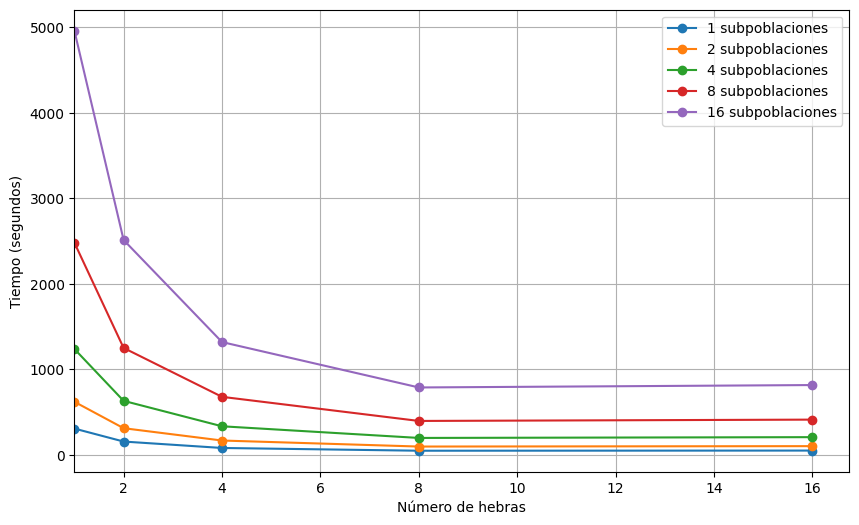
\includegraphics[width=0.8\textwidth]{imagenes/cap5/exploratory_subpopulations.png}
    \caption{Resultados de las ejecuciones exploratorias variando el número de subpoblaciones y hebras.}
    \label{fig:exploratory_subpopulations}
\end{figure}

\begin{table}[ht]
    \centering
    \begin{tabular}{|c|ccccc|}
        \hline
        \multirow{2}{*}{\textbf{Hebras}} & \multicolumn{5}{c|}{\textbf{Subpoblaciones}}                                                      \\ \cline{2-6}
                                         & \textbf{1}                                   & \textbf{2} & \textbf{4} & \textbf{8} & \textbf{16} \\ \hline
        1                                & 309.43                                       & 622.63     & 1239.73    & 2481.89    & 4960.00     \\ \hline
        2                                & 157.79                                       & 313.86     & 633.66     & 1252.12    & 2513.72     \\ \hline
        4                                & 82.73                                        & 169.76     & 336.25     & 680.46     & 1320.66     \\ \hline
        8                                & 50.58                                        & 99.37      & 200.01     & 398.66     & 790.04      \\ \hline
        16                               & 52.32                                        & 104.06     & 209.17     & 414.11     & 818.17      \\ \hline
    \end{tabular}
    \caption{Tiempos de ejecución en segundos para distintas combinaciones de hebras y subpoblaciones}
    \label{tab:exploratory_subpopulations_times}
\end{table}

\begin{table}[ht]
    \centering
    \begin{tabular}{|c|ccccc|}
        \hline
        \multirow{2}{*}{\textbf{Hebras}} & \multicolumn{5}{c|}{\textbf{Subpoblaciones}}                                                      \\ \cline{2-6}
                                         & \textbf{1}                                   & \textbf{2} & \textbf{4} & \textbf{8} & \textbf{16} \\ \hline
        1                                & 0.00                                         & 0.00       & 0.00       & 0.00       & 0.00        \\ \hline
        2                                & -49.01                                       & -49.59     & -48.89     & -49.55     & -49.32      \\ \hline
        4                                & -73.26                                       & -72.74     & -72.88     & -72.58     & -73.37      \\ \hline
        8                                & -83.65                                       & -84.04     & -83.87     & -83.94     & -84.07      \\ \hline
        16                               & -83.09                                       & -83.29     & -83.13     & -83.31     & -83.50      \\ \hline
    \end{tabular}
    \caption{Porcentaje de reducción del tiempo de ejecución respecto a la configuración base para distintas combinaciones de hebras y subpoblaciones}
    \label{tab:exploratory_populations_delta}
\end{table}

\subsection{Estudio del rendimiento al requerir más hebras de las disponibles}

En las figuras \ref{fig:exploratory_threads_1node}, \ref{fig:exploratory_threads_2nodes}, \ref{fig:exploratory_threads_4nodes}, \ref{fig:exploratory_threads_8nodes} y \ref{fig:exploratory_threads_16nodes} se presentan los resultados de las ejecuciones exploratorias correspondientes a configuraciones de 1, 2, 4, 8 y 16 nodos, respectivamente. Cada gráfica ilustra la evolución del tiempo de ejecución en función del número de hebras asignadas por nodo, diferenciando entre escenarios en los que el número total de hebras solicitadas se mantiene dentro del límite físico de 16 hebras del sistema y aquellos en los que dicho límite es excedido.

Por otro lado, en las figuras \ref{fig:exploratory_threads_1node_cpu}, \ref{fig:exploratory_threads_2nodes_cpu}, \ref{fig:exploratory_threads_4nodes_cpu}, \ref{fig:exploratory_threads_8nodes_cpu} y \ref{fig:exploratory_threads_16nodes_cpu} se muestran las gráficas correspondientes al uso de CPU para las mismas configuraciones de nodos y hebras por nodo.

\begin{figure}[ht]
    \centering
    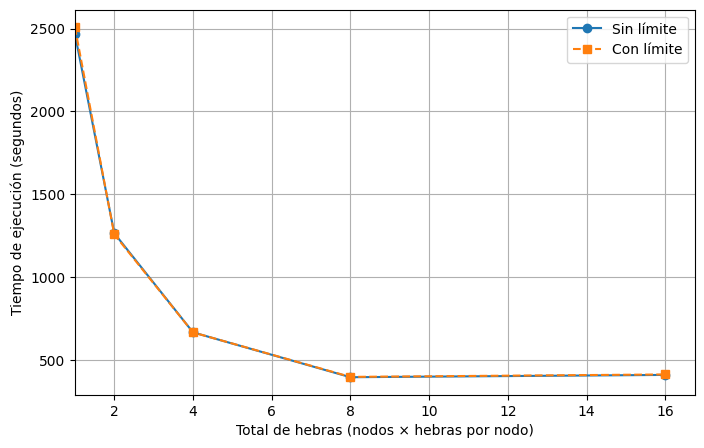
\includegraphics[width=0.8\textwidth]{imagenes/cap5/exploratory_threads_1node.png}
    \caption{Tiempo de ejecución en ejecuciones exploratorias con 1 nodo variando el número de hebras por nodo.}
    \label{fig:exploratory_threads_1node}
\end{figure}

\begin{figure}[ht]
    \centering
    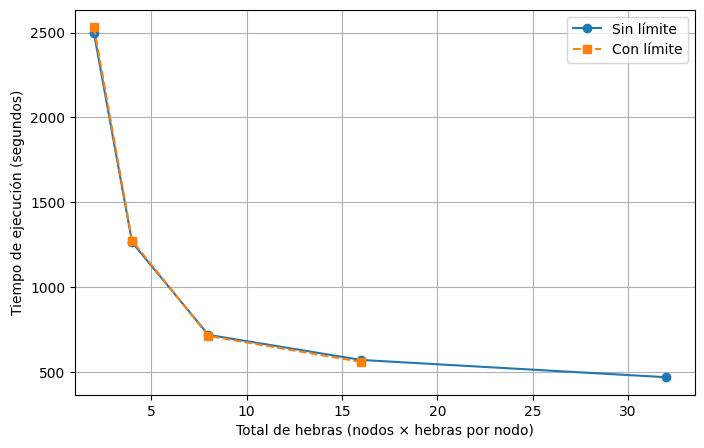
\includegraphics[width=0.8\textwidth]{imagenes/cap5/exploratory_threads_2nodes.png}
    \caption{Tiempo de ejecución en ejecuciones exploratorias con 2 nodos variando el número de hebras por nodo.}
    \label{fig:exploratory_threads_2nodes}
\end{figure}

\begin{figure}[ht]
    \centering
    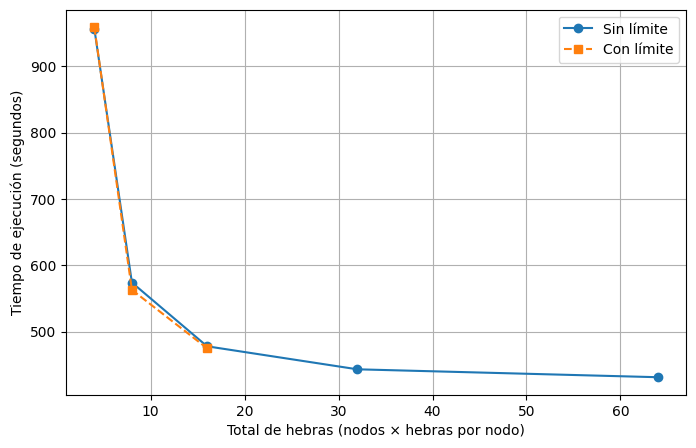
\includegraphics[width=0.8\textwidth]{imagenes/cap5/exploratory_threads_4nodes.png}
    \caption{Tiempo de ejecución en ejecuciones exploratorias con 4 nodos variando el número de hebras por nodo.}
    \label{fig:exploratory_threads_4nodes}
\end{figure}

\begin{figure}[ht]
    \centering
    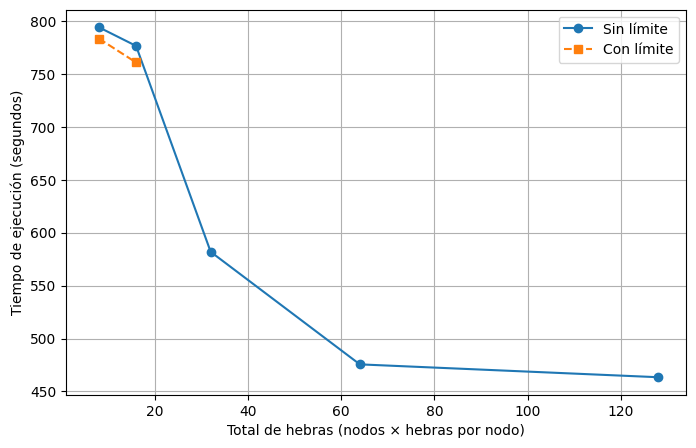
\includegraphics[width=0.8\textwidth]{imagenes/cap5/exploratory_threads_8nodes.png}
    \caption{Tiempo de ejecución en ejecuciones exploratorias con 8 nodos variando el número de hebras por nodo.}
    \label{fig:exploratory_threads_8nodes}
\end{figure}

\begin{figure}[ht]
    \centering
    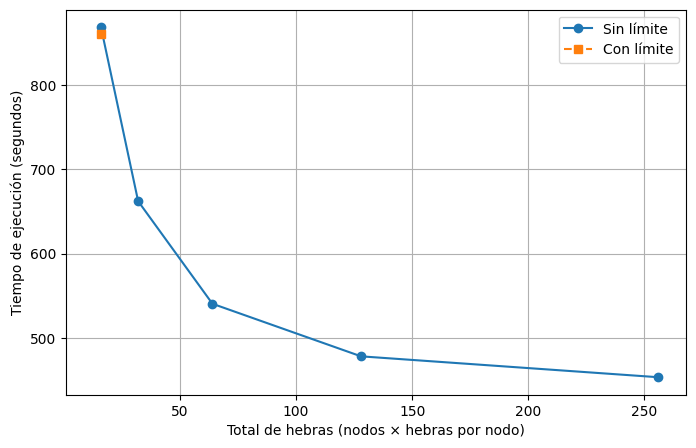
\includegraphics[width=0.8\textwidth]{imagenes/cap5/exploratory_threads_16nodes.png}
    \caption{Tiempo de ejecución en ejecuciones exploratorias con 16 nodos variando el número de hebras por nodo.}
    \label{fig:exploratory_threads_16nodes}
\end{figure}

\begin{figure}[ht]
    \centering
    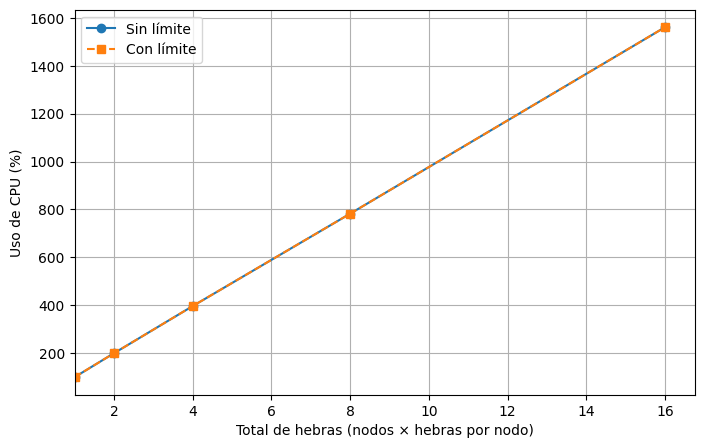
\includegraphics[width=0.8\textwidth]{imagenes/cap5/exploratory_threads_1node_cpu.png}
    \caption{Ejecuciones exploratorias con 1 nodo variando el número de hebras por nodo (uso de CPU).}
    \label{fig:exploratory_threads_1node_cpu}
\end{figure}

\begin{figure}[ht]
    \centering
    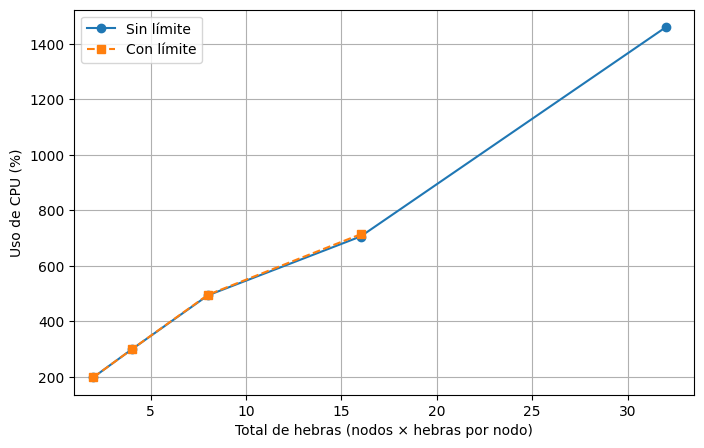
\includegraphics[width=0.8\textwidth]{imagenes/cap5/exploratory_threads_2nodes_cpu.png}
    \caption{Ejecuciones exploratorias con 2 nodos variando el número de hebras por nodo (uso de CPU).}
    \label{fig:exploratory_threads_2nodes_cpu}
\end{figure}

\begin{figure}[ht]
    \centering
    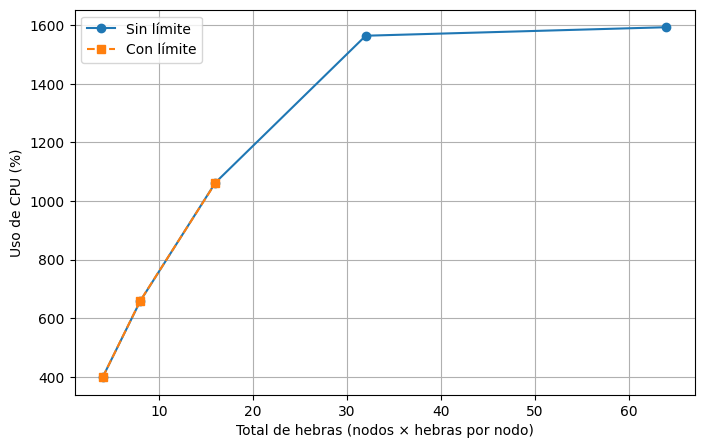
\includegraphics[width=0.8\textwidth]{imagenes/cap5/exploratory_threads_4nodes_cpu.png}
    \caption{Ejecuciones exploratorias con 4 nodos variando el número de hebras por nodo (uso de CPU).}
    \label{fig:exploratory_threads_4nodes_cpu}
\end{figure}

\begin{figure}[ht]
    \centering
    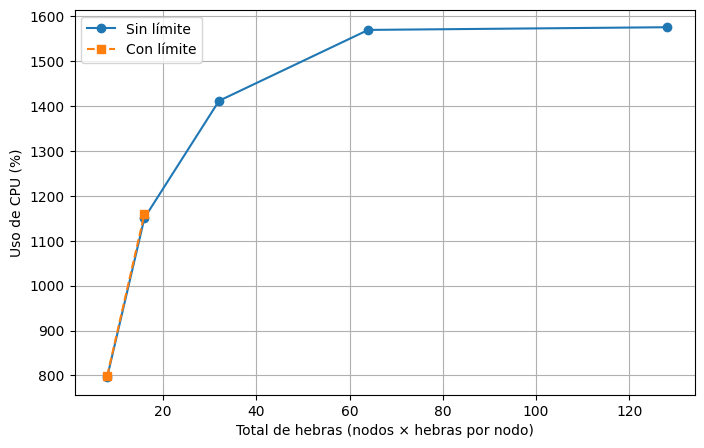
\includegraphics[width=0.8\textwidth]{imagenes/cap5/exploratory_threads_8nodes_cpu.png}
    \caption{Ejecuciones exploratorias con 8 nodos variando el número de hebras por nodo (uso de CPU).}
    \label{fig:exploratory_threads_8nodes_cpu}
\end{figure}

\begin{figure}[ht]
    \centering
    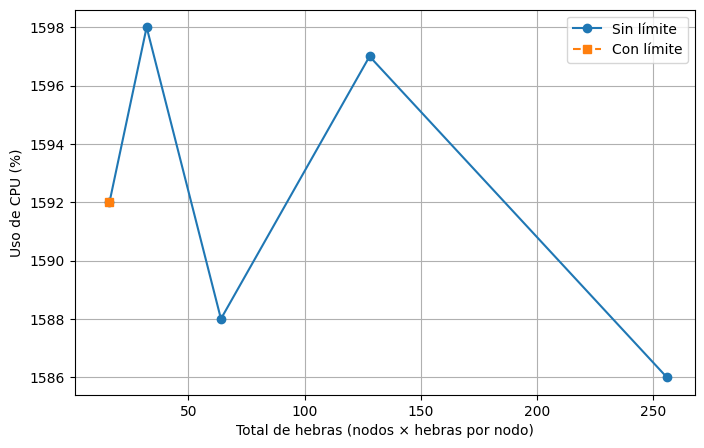
\includegraphics[width=0.8\textwidth]{imagenes/cap5/exploratory_threads_16nodes_cpu.png}
    \caption{Ejecuciones exploratorias con 16 nodos variando el número de hebras por nodo (uso de CPU).}
    \label{fig:exploratory_threads_16nodes_cpu}
\end{figure}

La información obtenida de estas gráficas se puede ver de forma más detallada y directa en la tabla \ref{tab:exploratory_all_nodes_threads}. En ella se presentan los tiempos de ejecución y el uso de CPU para todas las combinaciones de nodos y hebras por nodo. Se observa lo siguiente:

\begin{table}[ht]
    \centering
    \begin{tabular}{c c c c c}
        \hline
        \textbf{Nodos} & \textbf{Hebras / nodo} & \textbf{Hebras totales} & \textbf{Tiempo (s)} & \textbf{Uso de CPU (\%)} \\
        \hline
        1              & 8                      & 8                       & 395.63              & 782                      \\
        1              & 16                     & 16                      & 409.51              & 1561                     \\
        4              & 16                     & 64                      & 431.30              & 1593                     \\
        4              & 8                      & 32                      & 443.23              & 1564                     \\
        16             & 16                     & 256                     & 453.48              & 1586                     \\
        8              & 16                     & 128                     & 463.45              & 1576                     \\
        2              & 16                     & 32                      & 469.88              & 1460                     \\
        8              & 8                      & 64                      & 475.59              & 1570                     \\
        4              & 4                      & 16                      & 477.90              & 1063                     \\
        16             & 8                      & 128                     & 478.23              & 1597                     \\
        16             & 4                      & 64                      & 540.54              & 1588                     \\
        2              & 8                      & 16                      & 571.65              & 706                      \\
        4              & 2                      & 8                       & 573.94              & 659                      \\
        8              & 4                      & 32                      & 581.91              & 1412                     \\
        16             & 2                      & 32                      & 662.10              & 1598                     \\
        1              & 4                      & 4                       & 666.51              & 396                      \\
        2              & 4                      & 8                       & 719.43              & 494                      \\
        8              & 2                      & 16                      & 776.44              & 1151                     \\
        8              & 1                      & 8                       & 794.09              & 796                      \\
        16             & 1                      & 16                      & 868.28              & 1592                     \\
        4              & 1                      & 4                       & 956.38              & 399                      \\
        2              & 2                      & 4                       & 1263.74             & 299                      \\
        1              & 2                      & 2                       & 1264.94             & 199                      \\
        1              & 1                      & 1                       & 2467.76             & 99                       \\
        2              & 1                      & 2                       & 2497.06             & 199                      \\
        \hline
    \end{tabular}
    \caption{Tiempos de ejecución y uso de CPU para todas las combinaciones de nodos y hebras por nodo.}
    \label{tab:exploratory_all_nodes_threads}
\end{table}

A partir del análisis de la tabla, se pueden extraer las siguientes conclusiones técnicas:

\begin{itemize}
    \item El mejor rendimiento se alcanza al emplear un menor número de nodos y un mayor número de hebras por nodo, siendo la configuración óptima la de 1 nodo y 8 hebras.
    \item Aunque el límite físico de hebras de la CPU es de 16, se observa que, entre los 10 mejores resultados, solo 3 respetan este límite. En los demás casos, incrementar el número de hebras más allá de la capacidad física de la CPU sigue proporcionando mejoras en el rendimiento. Este comportamiento, aunque inicialmente contraintuitivo, puede explicarse analizando el uso efectivo de la CPU.
    \item El porcentaje de uso de CPU refleja el grado de aprovechamiento de las hebras disponibles. Por ejemplo, con 1 hebra el uso máximo es 100\%, con 2 hebras es 200\%, y así sucesivamente, hasta un máximo teórico de 1600\% (16 hebras $\times$ 100\%). En configuraciones con un único nodo, el incremento en el número de hebras se traduce en un aumento proporcional del uso de CPU:
\end{itemize}

\begin{table}[ht]
    \centering
    \begin{tabular}{|c|c|c|c|c|}
        \hline
        \textbf{Nodos} & \textbf{Hebras por nodo} & \textbf{Hebras totales} & \textbf{Tiempo (s)} & \textbf{Uso CPU (\%)} \\
        \hline
        1              & 8                        & 8                       & 395.63              & 782                   \\
        1              & 16                       & 16                      & 409.51              & 1561                  \\
        1              & 4                        & 4                       & 666.51              & 396                   \\
        1              & 2                        & 2                       & 1264.94             & 199                   \\
        1              & 1                        & 1                       & 2467.76             & 99                    \\
        \hline
    \end{tabular}
    \caption{Evolución del uso de CPU y tiempo de ejecución en configuraciones mononodo.}
\end{table}

\begin{itemize}
    \item En contraste, cuando el número total de hebras se distribuye entre varios nodos (incluso si no se supera el límite físico de la CPU), el rendimiento no mejora de la misma manera. Esto se debe a la sobrecarga asociada a la gestión de múltiples nodos, que puede contrarrestar los beneficios de disponer de más hebras. En estos casos, el uso de CPU no alcanza los valores esperados, resultando en un rendimiento inferior respecto a configuraciones mononodo equivalentes:
\end{itemize}

\begin{table}[ht]
    \centering
    \begin{tabular}{|c|c|c|c|c|}
        \hline
        \textbf{Nodos} & \textbf{Hebras por nodo} & \textbf{Hebras totales} & \textbf{Tiempo (s)} & \textbf{Uso CPU (\%)} \\
        \hline
        4              & 4                        & 16                      & 477.90              & 1063                  \\
        2              & 8                        & 16                      & 571.65              & 706                   \\
        4              & 2                        & 8                       & 573.94              & 659                   \\
        2              & 4                        & 8                       & 719.43              & 494                   \\
        8              & 2                        & 16                      & 776.44              & 1151                  \\
        8              & 1                        & 8                       & 794.09              & 796                   \\
        16             & 1                        & 16                      & 868.28              & 1592                  \\
        4              & 1                        & 4                       & 956.38              & 399                   \\
        2              & 2                        & 4                       & 1263.74             & 299                   \\
        2              & 1                        & 2                       & 2497.06             & 199                   \\
        \hline
    \end{tabular}
    \caption{Comparativa de rendimiento y uso de CPU en configuraciones multinodo.}
\end{table}

\begin{itemize}
    \item Por tanto, para configuraciones multinodo, es necesario incrementar el número de hebras más allá de la capacidad física de la CPU para acercarse al uso máximo teórico (1600\%), lo que explica por qué se obtienen mejores resultados bajo estas condiciones.
\end{itemize}

\subsection{Estudio del rendimiento al utilizar la misma GPU en distintos nodos}

En las figuras \ref{fig:exploratory_gpu_1node}, \ref{fig:exploratory_gpu_2nodes}, \ref{fig:exploratory_gpu_4nodes}, \ref{fig:exploratory_gpu_8nodes} y \ref{fig:exploratory_gpu_16nodes} se presentan los resultados de las ejecuciones exploratorias correspondientes a configuraciones de 1, 2, 4, 8 y 16 nodos, respectivamente. En ellas se muestra la evolución del tiempo de ejecución en función del número de hebras asignadas por nodo, diferenciando entre escenarios en los que todos los nodos utilizan la misma GPU y aquellos en los que solo un nodo hace uso de la GPU, mientras que los demás dependen exclusivamente de la CPU.

\begin{figure}[ht]
    \centering
    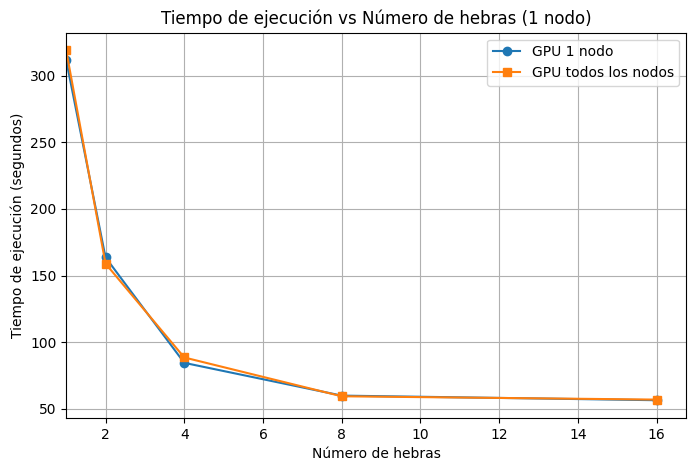
\includegraphics[width=0.8\textwidth]{imagenes/cap5/exploratory_gpu_1node.png}
    \caption{Gráfica de tiempo de ejecución con y sin GPU en ejecuciones con 1 nodo.}
    \label{fig:exploratory_gpu_1node}
\end{figure}

\begin{figure}[ht]
    \centering
    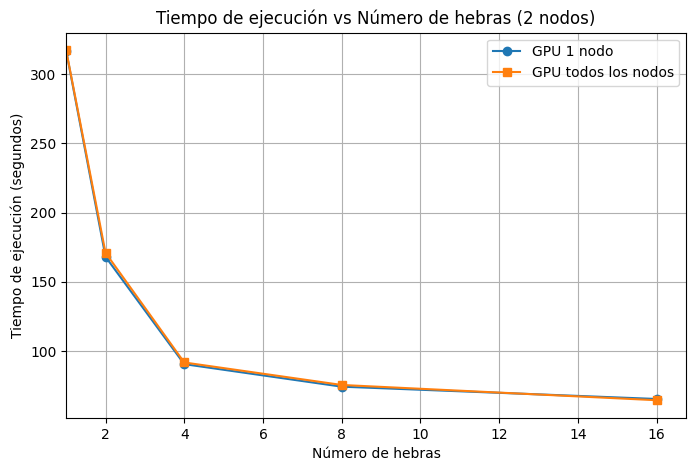
\includegraphics[width=0.8\textwidth]{imagenes/cap5/exploratory_gpu_2nodes.png}
    \caption{Gráfica de tiempo de ejecución con y sin GPU en ejecuciones con 2 nodos.}
    \label{fig:exploratory_gpu_2nodes}
\end{figure}

\begin{figure}[ht]
    \centering
    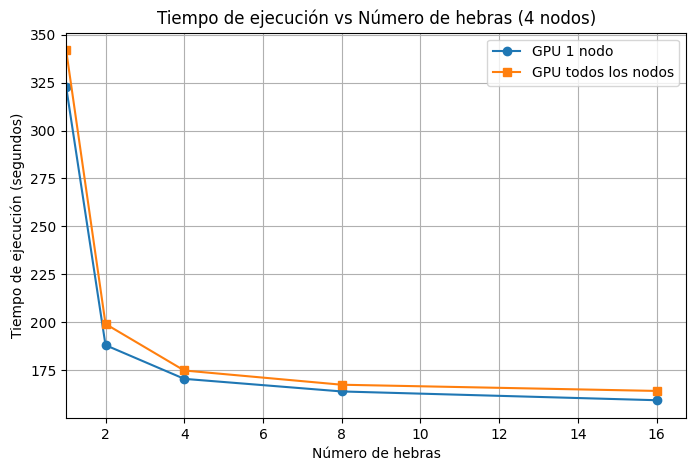
\includegraphics[width=0.8\textwidth]{imagenes/cap5/exploratory_gpu_4nodes.png}
    \caption{Gráfica de tiempo de ejecución con y sin GPU en ejecuciones con 4 nodos.}
    \label{fig:exploratory_gpu_4nodes}
\end{figure}

\begin{figure}[ht]
    \centering
    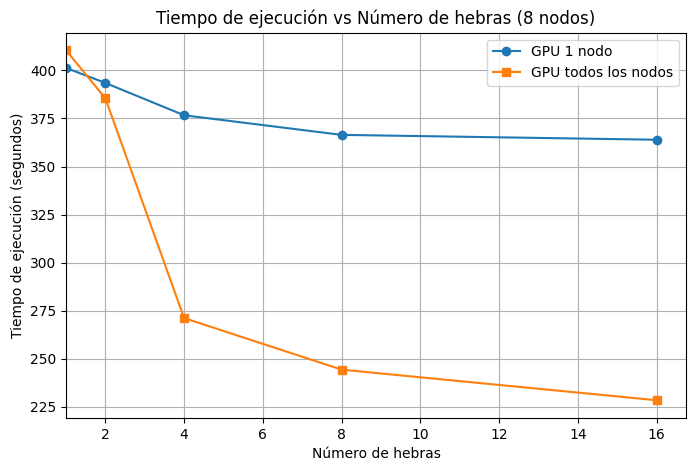
\includegraphics[width=0.8\textwidth]{imagenes/cap5/exploratory_gpu_8nodes.png}
    \caption{Gráfica de tiempo de ejecución con y sin GPU en ejecuciones con 8 nodos.}
    \label{fig:exploratory_gpu_8nodes}
\end{figure}

\begin{figure}[ht]
    \centering
    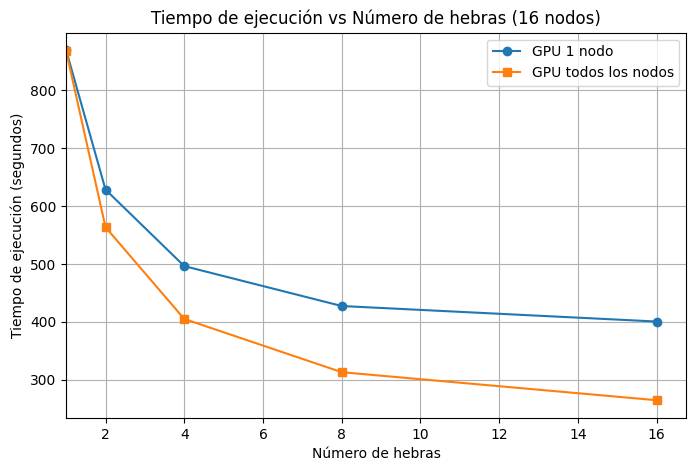
\includegraphics[width=0.8\textwidth]{imagenes/cap5/exploratory_gpu_16nodes.png}
    \caption{Gráfica de tiempo de ejecución con y sin GPU en ejecuciones con 16 nodos.}
    \label{fig:exploratory_gpu_16nodes}
\end{figure}

\begin{table}[ht]
    \centering
    \begin{tabular}{c|ccc}
        Hebras & GPU 1 nodo (s) & GPU todos los nodos (s) & $\Delta$ (\%) \\
        \hline
        1.00   & 311.68         & 319.01                  & 2.35          \\
        2.00   & 163.59         & 158.94                  & -2.84         \\
        4.00   & 84.49          & 88.52                   & 4.77          \\
        8.00   & 59.91          & 59.41                   & -0.83         \\
        16.00  & 56.45          & 56.91                   & 0.81          \\
    \end{tabular}
    \caption{Tiempos de ejecución en 1 nodo comparando GPU en 1 nodo versus GPU en todos los nodos.}
    \label{tab:gpu_1node}
\end{table}

\begin{table}[ht]
    \centering
    \begin{tabular}{c|ccc}
        Hebras & GPU 1 nodo (s) & GPU todos los nodos (s) & $\Delta$ (\%) \\
        \hline
        1.00   & 316.92         & 317.35                  & 0.14          \\
        2.00   & 168.14         & 170.99                  & 1.70          \\
        4.00   & 90.58          & 91.78                   & 1.32          \\
        8.00   & 74.30          & 75.53                   & 1.66          \\
        16.00  & 65.40          & 64.51                   & -1.36         \\
    \end{tabular}
    \caption{Tiempos de ejecución en 2 nodos comparando GPU en 1 nodo versus GPU en todos los nodos.}
    \label{tab:gpu_2nodes}
\end{table}

\begin{table}[ht]
    \centering
    \begin{tabular}{c|ccc}
        Hebras & GPU 1 nodo (s) & GPU todos los nodos (s) & $\Delta$ (\%) \\
        \hline
        1.00   & 322.77         & 341.95                  & 5.94          \\
        2.00   & 187.98         & 199.04                  & 5.88          \\
        4.00   & 170.38         & 174.74                  & 2.56          \\
        8.00   & 163.80         & 167.31                  & 2.14          \\
        16.00  & 159.22         & 164.07                  & 3.05          \\
    \end{tabular}
    \caption{Tiempos de ejecución en 4 nodos comparando GPU en 1 nodo versus GPU en todos los nodos.}
    \label{tab:gpu_4nodes}
\end{table}

\begin{table}[ht]
    \centering
    \begin{tabular}{c|ccc}
        Hebras & GPU 1 nodo (s) & GPU todos los nodos (s) & $\Delta$ (\%) \\
        \hline
        1.00   & 401.33         & 410.54                  & 2.29          \\
        2.00   & 393.50         & 385.47                  & -2.04         \\
        4.00   & 376.68         & 271.10                  & -28.03        \\
        8.00   & 366.47         & 244.26                  & -33.35        \\
        16.00  & 363.94         & 228.34                  & -37.26        \\
    \end{tabular}
    \caption{Tiempos de ejecución en 8 nodos comparando GPU en 1 nodo versus GPU en todos los nodos.}
    \label{tab:gpu_8nodes}
\end{table}

\begin{table}[ht]
    \centering
    \begin{tabular}{c|ccc}
        Hebras & GPU 1 nodo (s) & GPU todos los nodos (s) & $\Delta$ (\%) \\
        \hline
        1.00   & 869.40         & 867.50                  & -0.22         \\
        2.00   & 628.49         & 563.51                  & -10.34        \\
        4.00   & 496.28         & 404.98                  & -18.40        \\
        8.00   & 427.30         & 312.94                  & -26.76        \\
        16.00  & 400.48         & 264.49                  & -33.96        \\
    \end{tabular}
    \caption{Tiempos de ejecución en 16 nodos comparando GPU en 1 nodo versus GPU en todos los nodos.}
    \label{tab:gpu_16nodes}
\end{table}

\subsection{Análisis y conclusiones}

\subsubsection{Análisis del rendimiento}

Para configuraciones de 1, 2 y 4 nodos, las diferencias de rendimiento entre las ejecuciones con límite de uso de GPU y sin límite son reducidas (\(\Delta\)\% entre -3\% y +6\%), sin observarse una tendencia sistemática a favor de una u otra opción. En estos casos, la variabilidad puede atribuirse a fluctuaciones experimentales y no a restricciones impuestas por el entorno.

No obstante, al incrementar el número de nodos a 8 y 16, la versión sin límite muestra una ventaja clara y consistente, alcanzando diferencias de hasta -37\% en el caso de 16 hebras y 16 nodos. Esto evidencia que la imposición de un límite restringe el aprovechamiento de los recursos disponibles, especialmente en escenarios de alta concurrencia y escalabilidad.

En consecuencia, para estudios de escalabilidad multinodo, se recomienda emplear la versión sin límite, ya que permite obtener tiempos de ejecución menores y refleja de manera más precisa el potencial máximo del sistema al aumentar el número de nodos y hebras.

\subsubsection{Conclusiones técnicas}

A partir de los experimentos realizados, se extraen las siguientes conclusiones relevantes para la configuración de los estudios posteriores:

\begin{itemize}
    \item \textbf{Número de subpoblaciones:} Se selecciona 8 subpoblaciones como valor óptimo, ya que maximiza el rendimiento observado. Utilizar menos subpoblaciones implica un aprovechamiento subóptimo de los recursos de cómputo, mientras que incrementarlas no aporta mejoras significativas, evidenciando que el sistema alcanza su máximo rendimiento con 8 subpoblaciones.

    \item \textbf{Número de hebras:} El incremento del número de hebras no garantiza una mejora continua del rendimiento, especialmente cuando estas se reparten en más nodos. El mejor resultado se obtiene con una configuración de 1 nodo y 8 hebras, coincidiendo con el número de núcleos físicos del sistema.

          \begin{itemize}
              \item \textbf{Diferencia porcentual de rendimiento:} La diferencia de tiempo de ejecución entre la configuración óptima (1 nodo, 8 hebras) y la de 1 nodo y 16 hebras es:
                    \[
                        \text{Diferencia (\%) } = \frac{409.51 - 395.63}{395.63} \times 100 \approx 3.51\mathrm{\%}
                    \]


                    Por tanto, ejecutar con 1 nodo y 16 hebras resulta aproximadamente un \textbf{3.5\% más lento} que con 1 nodo y 8 hebras.

              \item \textbf{Criterio para estudios comparativos:} Dado que el objetivo principal es comparar la conservación del rendimiento entre la ejecución nativa y la ejecución en contenedores, y no la búsqueda del óptimo absoluto, se realizarán los experimentos mononodo hasta 16 hebras.

              \item \textbf{Escalabilidad multinodo:} Para el análisis multinodo, se mantendrá el criterio de comparar el rendimiento observado en la ejecución nativa, explorando configuraciones de hasta 16 nodos y 16 hebras, asegurando así una evaluación completa de la escalabilidad y la equivalencia de rendimiento entre ambos entornos.
          \end{itemize}

    \item \textbf{Uso de GPU:} En pruebas de rendimiento en entornos que utilizan GPU, esta estará disponible en todos los nodos. Esto se debe a que se ha demostrado que el rendimiento es superior cuando la GPU está a disposición de todos los nodos, especialmente en escenarios de alta concurrencia y escalabilidad.
\end{itemize}




\section{Pruebas mononodo}
\subsection{Ejecución en Ubuntu en nativo}
\paragraph{CPU}

\paragraph{CPU + GPU}

\subsection{Ejecución en contenedores de Ubuntu}
\paragraph{CPU}

\paragraph{CPU + GPU}

\subsection{Contenedores en contenedores de Windows}
\paragraph{CPU}

\paragraph{CPU + GPU}

\subsection{Contenedores en contenedores de Mac}
\paragraph{CPU}

\section{Pruebas multinodo}
\subsection{Ejecución en Ubuntu en nativo}
\paragraph{CPU}

\paragraph{CPU + GPU}

\subsection{Ejecución en contenedores de Ubuntu}
\paragraph{CPU}

\paragraph{CPU + GPU}

\subsection{Contenedores en contenedores de Windows}
\paragraph{CPU}

\paragraph{CPU + GPU}

\subsection{Contenedores en contenedores de Mac}
\paragraph{CPU}

\section{Pruebas de barrido de hebras}
\subsection{Ejecución en Ubuntu en nativo}
\paragraph{CPU}

\paragraph{CPU + GPU}

\subsection{Ejecución en contenedores de Ubuntu}
\paragraph{CPU}

\paragraph{CPU + GPU}

\subsection{Contenedores en contenedores de Windows}
\paragraph{CPU}

\paragraph{CPU + GPU}

\subsection{Contenedores en contenedores de Mac}
\paragraph{CPU}

